\documentclass{beamer}

\mode<presentation>{%
\usetheme{Warsaw} %{Berkeley}
% \usecolortheme{dolphin}
\setbeamercovered{transparent} 
\setbeamertemplate{navigation symbols}{}
}

% Definições latex para portugues
\usepackage[utf8]{inputenc}
\usepackage[brazil]{babel}
\usepackage[T1]{fontenc}

% Formatação de URL
\usepackage{url}

% Adição de figuras no documento
\usepackage{graphicx}
\usepackage{setspace}
\usepackage{graphics}

% Definições matemáticas
\usepackage{amsmath}
\usepackage{amsfonts}

% Tabelas longas (mais de uma página)
\usepackage{longtable}
\usepackage{rotating}
\usepackage{array}
\usepackage{multirow}

% definicoes
\newtheorem{teo}{Teorema}
\newtheorem{defin}{Definição}

%  ABACO -- Conjunto de macros para desenhar o 'abaco

%  Desenho original de Hans Liesenberg

%  Macros de Tomasz Kowaltowski

%  DCC -- IMECC -- UNICAMP

%  Mar,co de 1988  --  Vers~ao 1.0

% Ajustado para LaTeX da SUN -- Mar,co de 1991

% ---------------------------------------------------------

%  Chamada:   \ABACO{d1}{d2}{d3}{d4}{esc}
%             com:  di's -- os quatro d'igitos;
%	           esc  -- fator de escala

% ---------------------------------------------------------

%  DEFINI,C~OES AUXILIARES

% ---------------------------------------------------------


%  Forma o d'igito pequeno (0 ou 1)

\newcommand{\ABACODP}[1]{%
%
\thicklines
%    
\begin{picture}(8,0)
    \ifcase#1{   %  caso 0
       \put(0,0)    {\line(1,0){4}}
       \multiput(5,0)(2,0){2}{\oval(2,4)}}
    \or{         %  caso 1
       \put(2,0)    {\line(1,0){4}}
       \multiput(1,0)(6,0){2}{\oval(2,4)}}
    \fi
\end{picture}
    } % \ABACODP

% Forma o d'igito grande (0 a 4)

\newcommand{\ABACODG}[1]{%
%
\thicklines
%    
\begin{picture}(14,0)
    \ifcase#1{   % caso 0
       \multiput(1,0)(2,0){5}{\oval(2,4)}}
       \put(10,0)   {\line(1,0){4}}
    \or{         % caso 1
       \multiput(1,0)(2,0){4}{\oval(2,4)}}
       \put(8,0)   {\line(1,0){4}}
       \put(13,0)   {\oval(2,4)}
    \or{         % caso 2
       \multiput(1,0)(2,0){3}{\oval(2,4)}
       \put(6,0)   {\line(1,0){4}}
       \multiput(11,0)(2,0){2}{\oval(2,4)}}
    \or{         % caso 3
       \multiput(1,0)(2,0){2}{\oval(2,4)}
       \put(4,0)   {\line(1,0){4}}
       \multiput(9,0)(2,0){3}{\oval(2,4)}}
    \or{         % caso 4
       \put(1,0)  {\oval(2,4)}}
       \put(2,0)   {\line(1,0){4}}
       \multiput(7,0)(2,0){4}{\oval(2,4)}
    \fi
\end{picture}
    } % \ABACODG
       
% Forma um d'igito (0 a 9)

\newcommand{\ABACOD}[1]{%
%
    \ifnum#1>9
       \errmessage{#1: Argumento invalido para ABACO}
    \fi
    \ifnum#1<0
       \errmessage{#1: Argumento invalido para ABACO}
    \fi
%
\begin{picture}(24,0)
%    
    \ifnum#1<5
       \put(16,0) {\ABACODP{0}}
    \else   
       \put(16,0) {\ABACODP{1}}
    \fi
%    
    \ifnum#1<5
       \put(0,0)  {\ABACODG{#1}}
    \else
       \ifcase#1\or \or \or \or
          \or  \put(0,0)  {\ABACODG{0}}
          \or  \put(0,0)  {\ABACODG{1}}
          \or  \put(0,0)  {\ABACODG{2}}
          \or  \put(0,0)  {\ABACODG{3}}
          \or  \put(0,0)  {\ABACODG{4}}
       \fi
    \fi   
\end{picture}
    } % \ABACOD
    
% -------------------------------------------------

%  DEFINI,C~AO PRINCIPAL
    
\newcommand{\ABACO}[5]{%
    \setlength{\unitlength}{#5mm}
%
    \thinlines
%   
\begin{picture}(28,25)
%   
% moldura
%
% externa
%
        \put(0,0)            {\line(0,1){25}}
        \put(0,0)            {\line(1,0){28}}
        \put(28,0)           {\line(0,1){25}}
        \put(0,25)           {\line(1,0){28}}
% interna
        \put(2,2)            {\line(0,1){21}}
	\put(26,2)           {\line(0,1){21}}
	\put(16,2)           {\line(0,1){21}}
	\put(18,2)           {\line(0,1){21}}
	\put(2,2)            {\line(1,0){14}}
	\put(16,2)           {\line(1,-1){1}}
	\put(17,1)           {\line(1,1){1}}
	\put(18,2)           {\line(1,0){8}}
	\put(2,23)           {\line(1,0){14}}
	\put(16,23)          {\line(1,1){1}}
	\put(17,24)          {\line(1,-1){1}}
	\put(18,23)          {\line(1,0){8}}
	\put(0,0)            {\line(1,1){2}}
	\put(0,25)           {\line(1,-1){2}}
	\put(28,0)           {\line(-1,1){2}}
	\put(28,25)          {\line(-1,-1){2}}
%
%   
% d'igitos
%
%   
       \put(2,20)  {\ABACOD{#1}}
       \put(2,15)  {\ABACOD{#2}}
       \put(2,10)  {\ABACOD{#3}}
       \put(2,5)   {\ABACOD{#4}}
%      
\end{picture}
    } % \ABACO
    


\defbeamertemplate*{footline}{shadow theme}
{%
    \leavevmode%
    \hbox{\begin{beamercolorbox}[wd=.5\paperwidth,ht=2.5ex,dp=1.125ex,leftskip=.3cm,rightskip=.3cm
        plus1fil]{title in head/foot}%
        \usebeamerfont{title in
        head/foot}\insertshorttitle%
    \end{beamercolorbox}%
    \begin{beamercolorbox}[wd=.5\paperwidth,ht=2.5ex,dp=1.125ex,leftskip=.3cm
        plus1fil,rightskip=.3cm]{author in head/foot}%
        \usebeamerfont{author in
        head/foot}\insertshortauthor\hfill\insertframenumber\,/\,\inserttotalframenumber
    \end{beamercolorbox}}%
}


\title[PR aplicada a Problemas de Rearranjo de Genomas]{Programação por
Restrições aplicada a Problemas de Rearranjo de Genomas}

\author[Victor de Abreu Iizuka and Zanoni Dias]{Victor de Abreu Iizuka\\ 
Orientador: Zanoni Dias}

\institute[UNICAMP]{\textbf{Instituto de Computação, Universidade Estadual
de Campinas}\\ \begin{columns}[t]
    \begin{column}{5cm}
        \vspace{-1.2cm}
        \begin{figure}
            \centering
            
\includegraphics[scale=0.4]{images/unicamp-logo.jpg}
        \end{figure} 
    \end{column}
    \begin{column}{5cm} 
        \parbox{1in}{\center{\ABACO{2}{0}{1}{2}{0.7}}}
    \end{column}
\end{columns}}

\date{}

\renewcommand{\raggedright}{\leftskip=0pt \rightskip=0pt plus 0cm} 

\begin{document}

% slide 1
\frame{\titlepage}

% slide 2
\frame{\tableofcontents}

\section{Introdução}

% slide 3
\frame{\frametitle{Introdução [1/3]}

\begin{itemize} 

    \item{Rearranjo de genomas tem como o objetivo encontrar o menor
        número de operações que transformam um genoma em outro.}

    \item{Essas operações podem ser reversões, transposições, fissões e
        fusões.}

    \item{Estudos mostram que rearranjos são mais adequados que mutações
        pontuais quando se deseja comparar os genomas de duas espécies
        [Palmer e Herbon (1988), Bafna e Pevzner~(1995)].}

\end{itemize}}

% slide 4
\frame{\frametitle{Introdução [2/3]}

\begin{itemize} 
    
    \item{Neste contexto, a distância evolutiva é o menor número de
        operações que são necessárias para transformar um genoma em
        outro.}

    \item{Neste trabalho, trataremos os casos em que os eventos de
        reversões e transposições ocorrem de forma isolada e os casos
        quando os dois eventos ocorrem ao mesmo tempo.}

    \item{O trabalho desenvolvido nesta dissertação segue a linha de
        pesquisa utilizada por Dias e Dias~(2009) e nós apresentaremos
        modelos de Programação por Restrições (PR/CP) para ordenação por
        reversões e ordenação por reversões e transposições, baseados na
        teoria do Problema de Satisfação de Restrições (PSR/CSP) e na teoria
        do Problema de Otimização com Restrições (POR/COP).}

\end{itemize}}

% slide 5
\frame{\frametitle{Introdução [3/3]}

\begin{itemize}

    \item{Nós fizemos comparações com os modelos de Programação por
        Restrições para ordenação por transposições, descrito por Dias e
        Dias~(2009), e no caso de ordenação por reversões e ordenação
        por reversões e transposições, com os modelos de Programação
        Linear Inteira (PLI/ILP) descritos por Dias e Souza~(2007).}

    \item{O artigo \textit{Constraint logic programming models for
        reversal and transposition distance problems} foi publicado no
        \textit{VI Brazilian Symposium on Bioinformatics} (BSB'2011).}

\end{itemize}}
%%% \end{Introdução} %%%

% slide 6
\frame{\frametitle{Permutação}

\begin{itemize}

    \item{Para fins computacionais, um genoma é representado por uma
        $n$-tupla de genes, e quando não há genes repetidos essa tupla é
        chamada de permutação.}

    \item{Uma permutação é representada como $\pi =
        (\pi_{1}~\pi_{2}~\ldots~\pi_{n})$, para $\pi_{i} \in
        \mathbb{N}$, $1 \leq \pi_{i} \leq n$ e $i \neq j \leftrightarrow
        \pi_{i} \neq \pi_{j}$.}

    \item{A permutação identidade é representada como $\iota =
        (1~2~3~\ldots~n)$.}
    
\end{itemize}} 

\subsection{Problema da Distância de Reversão} 

% slide 7
\frame{\frametitle{Problema da Distância de Reversão [1/2]} 

\begin{beamerboxesrounded}[center,shadow=true]{Evento de reversão:} 
    \footnotesize
    Um evento de reversão ocorre quando um bloco do genoma é invertido.
    \normalsize
\end{beamerboxesrounded} 

\begin{columns}[t] 
    \begin{column}{5cm} 
        \begin{figure}
            \centering 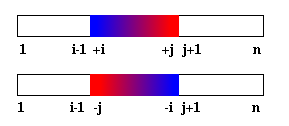
\includegraphics[width=4.5cm]{images/rev02.png}
            \caption{Uma reversão aplicada sobre uma permutação
            orientada.}
        \end{figure} 
    \end{column}
    \begin{column}{5cm} 
        \begin{figure} 
            \centering
            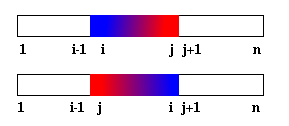
\includegraphics[width=4.5cm]{images/rev01.png} 
            \caption{Uma~reversão~aplicada~sobre uma permutação não
            orientada.} 
        \end{figure} 
    \end{column}
\end{columns} }

% slide 8
\frame{\frametitle{Problema da Distância de Reversão [2/2]} 

\begin{itemize} 
    
    \item{O Problema da Distância de Reversão é encontrar o número
        mínimo de reversões necessárias para transformar uma genoma em
        outro.}

    \item{O Problema da Distância de Reversão é equivalente ao problema de
        Ordenação por Reversões, que é a distância de reversão entre a
        permutação $\pi$ e a permutação identidade $\iota$, denotado por
        $d_{r}(\pi)$.}

    \item{Se a orientação dos genes é conhecida, o problema pode ser
        solucionado com algoritmos polinomiais.}

    \item{Caso contrário, o problema pertence à classe de problemas
        NP-Difíceis, com a prova apresentada por Caprara (1997).}  

    \item{Melhor algoritmo de aproximação possui razão de $1.375$ e foi
        apresentado por Berman, Hannenhalli e Karpinski (2002).}

\end{itemize} }

% slide 9
\frame{\frametitle{Grafo de Breakpoints para Reversões [1/4]} 

\begin{beamerboxesrounded}[center,shadow=true]{Breakpoints:}  
    \footnotesize
    Dois elementos consecutivos $\pi_{i}$ e $\pi_{i+1}$, $0 \le i \le
    n$, são \textit{adjacentes} quando $|\pi_{i} - \pi_{i+1}| = 1$, e
    são \textit{breakpoints} caso contrário. 
    \normalsize
\end{beamerboxesrounded}

\begin{itemize} 
    
    \item{A permutação $\pi$ é estendida adicionando os elementos
        $\pi_{0} = 0$ e $\pi_{n+1} = n+1$.}

    \item{Grafo de arestas coloridas $G(\pi)$ com $n+2$ vértices \{$0,
        1,~\ldots~, n, \newline n+1$\}.}

    \item{Uma aresta preta liga os vértices $i$ e $j$ se $(i, j)$ for um
        \textit{breakpoint}.}

    \item{Uma aresta cinza liga os vértices $i$ e $j$ se $|i - j| = 1$ e
        os dois não são consecutivos em $\pi$.}

\end{itemize} }

% slide 10
\frame{\frametitle{Grafo de Breakpoints para Reversões [2/4]} 

\begin{columns}[t]
    \begin{column}{5cm}
        \begin{figure}
            \centering
            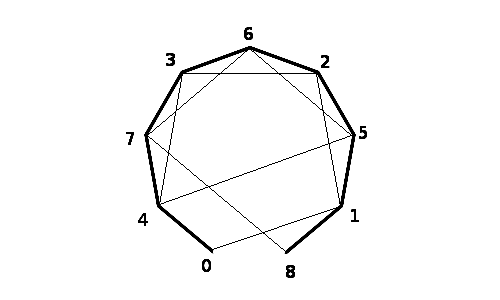
\includegraphics[width=5cm]{images/rev_grafo_bkp.png}
            \caption{Grafo de \textit{Breakpoints} da permutação $\pi =
        (4~7~3~6~2~5~1)$}
        \end{figure}
        \vspace{1cm}
    \end{column}
    \begin{column}{5cm}
        \begin{itemize}
            
            \footnotesize
            \item{Reversão atua em dois pontos em uma permutação,
                    portanto pode reduzir o número de breakpoints em
                    pelo menos um e no máximo dois.}
            \normalsize

        \end{itemize}
        
        \vspace{0.8cm}

        \begin{beamerboxesrounded}[center,shadow=true]{Teorema 1:}
            \footnotesize
            Para qualquer permutação $\pi$, 
            \[\frac{1}{2} b_r(\pi) \leq d_r(\pi) \leq
                b_r(\pi).
            \]
            \normalsize
        \end{beamerboxesrounded}
    \end{column}
\end{columns} }

% slide 11
\frame{\frametitle{Grafo de Breakpoints para Reversões [3/4]}

\begin{figure}[h]
    \centering 
    \begin{tabular}{ccc} 
        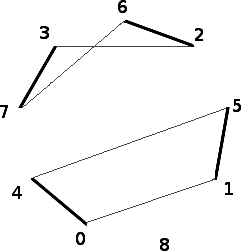
\includegraphics[scale=0.35]{images/rev_grafo_bkp_dec2cic-1.png}
        & ~~~~
        & 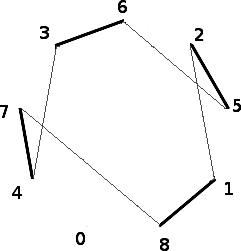
\includegraphics[scale=0.35]{images/rev_grafo_bkp_dec2cic-2.png} 
    \end{tabular} 
    \caption{Exemplo de decomposição em ciclos de arestas disjuntas para
        o grafo de \textit{breakpoints} da permutação $\pi =
    (4~7~3~6~2~5~1)$.}
\end{figure} }

% slide 12
\frame{\frametitle{Grafo de Breakpoints para Reversões [4/4]}

\begin{itemize}

    \item{O grafo pode ser decomposto em ciclos de arestas disjuntas.}

    \item{Existem diversas maneiras de realizar a decomposição.}

    \item{O Teorema 2, demonstrado no trabalho de Christie (1998),
          fornece os limitantes para a distância de reversão usando a
          quantidade de 2-ciclos na máxima decomposição de ciclos de
          $G(\pi)$.}

\end{itemize}

\vspace{0.5cm}

\begin{beamerboxesrounded}[center,shadow=true]{Teorema 2:}
    \footnotesize
    Se $c_{2}(\pi)$ é o número mínimo de $2$-ciclos em qualquer máxima
    decomposição em ciclos de $G(\pi)$ então: 
    \[
        \frac{2}{3} b_r(\pi)
        - \frac{1}{3} c_{2}(\pi) \leq d_r(\pi) \leq b_r(\pi) - \frac{1}{2}
        c_{2}(\pi).
    \]
    \normalsize
\end{beamerboxesrounded} }

\subsection{Problema da Distância de Transposição} 

% slide 13
\frame{\frametitle{Problema da Distância de Transposição [1/2]}

\begin{beamerboxesrounded}[center,shadow=true]{Evento de transposição:} 
    Um evento de transposição ocorre quando dois blocos adjacentes no
    genoma trocam de posição.
\end{beamerboxesrounded} 

\begin{figure} 
    \centering
    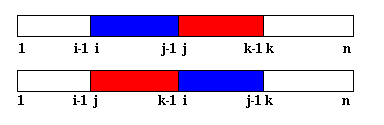
\includegraphics[width=6cm]{images/transv.png} 
    \caption{Uma transposição aplicada em uma permutação.}
\end{figure} }

% slide 14
\frame{\frametitle{Problema da Distância de Transposição [2/2]}

\begin{itemize}

    \item{O Problema da Distância de Transposição é encontrar o número
        mínimo de transposições necessárias para transformar um genoma em
        outro.} 

    \item{O Problema da Distância de Transposição é equivalente ao
        problema de Ordenação por Transposições, que é a distância
        de transposição entre a permutação $\pi$ e a permutação
        identidade $\iota$, denotado por $d_{t}(\pi)$.}

    \item{Pertence à classe de problemas NP-Difíceis, a prova foi
        apresentada por Bulteau, Fertin e Rusu (2010).} 

    \item{O melhor algoritmo de aproximação possui razão de $1.375$ e
        foi apresentado por Elias e Hartman (2006).} 

\end{itemize} }

% slide 15
\frame{\frametitle{Breakpoints para Transposições} 

\begin{beamerboxesrounded}[center,shadow=true]{Breakpoints:}  
    \footnotesize
    Um \textit{breakpoint} é um par $(\pi_{i}, \pi_{i+1})$, tal que
    $\pi_{i+1} \neq \pi_{i} + 1$. 
    \normalsize
\end{beamerboxesrounded}

\begin{itemize} 
    
    \item{A permutação $\pi$ é estendida adicionando os elementos
        $\pi_{0} = 0$ e $\pi_{n+1} = n+1$.}

    \item{Uma transposição atua em três pontos de uma permutação, logo
        pode reduzir o número de \textit{breakpoints} em pelo menos
        e no máximo três.}

\end{itemize} 

\begin{beamerboxesrounded}[center,shadow=true]{Teorema 3:}
    \footnotesize
    Para qualquer permutação $\pi$, 
    \[\frac{1}{3} b_t(\pi) \leq d_t(\pi) \leq
        b_t(\pi).
    \]
    \normalsize
\end{beamerboxesrounded} }

% slide 16
\frame{\frametitle{Grafo de Ciclos [1/3]}

\begin{itemize}

    \item{Introduzido por Bafna e Pevzner (1998).}

    \item{Grafo direcionado com arestas coloridas $G(\pi)$ com $n+2$
          vértices $\{0,~1,~\ldots,~n,~n+1\}$.}

    \item{Arestas cinzas são direcionadas de $i-1$ para $i$.}

    \item{Arestas pretas são direcionadas de $\pi_i$ para $\pi_{i-1}$.}

\end{itemize} 

\begin{figure}
    \centering
    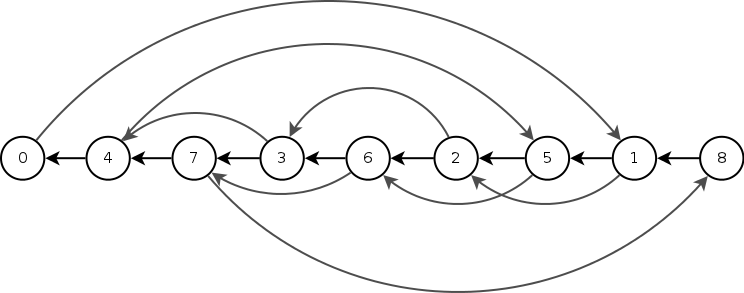
\includegraphics[width=8cm]{images/trans_cycle_graph.png}
    \caption{Grafo de ciclos da permutação $\pi = (4~7~3~6~2~5~1)$}
\end{figure} }

% slide 17
\frame{\frametitle{Grafo de Ciclos [2/3]}

\begin{figure}[h]
  \centering 
  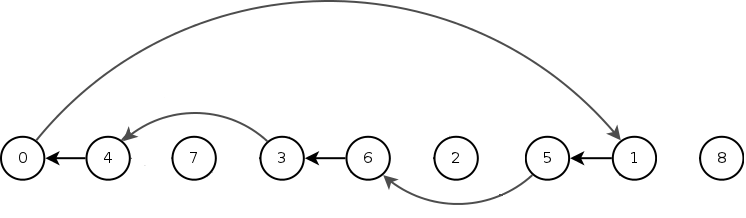
\includegraphics[width=8cm,height=2.4cm]{images/trans_cycle_graph_dec-1.png}
  \vspace{0.0001cm}
  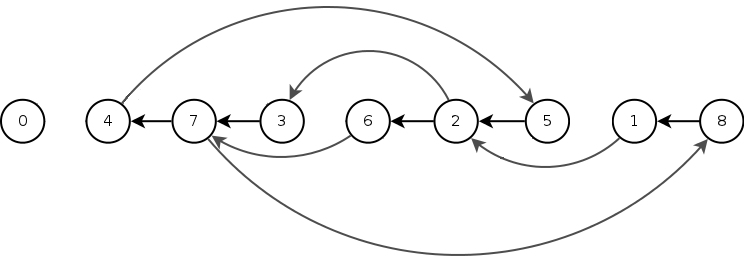
\includegraphics[width=8cm,height=2.8cm]{images/trans_cycle_graph_dec-2.png} 
  \caption{Exemplo de decomposição em ciclos de arestas disjuntas para
  o grafo de ciclos da permutação $\pi = (4~7~3~6~2~5~1)$.}
  \label{fig:tra_grafo_bkp_dec}
\end{figure} }

% slide 18
\frame{\frametitle{Grafo de Ciclos [3/3]}

\begin{itemize}

    \item{Para todo vértice de $G(\pi)$ toda aresta chegando é
        unicamente pareada com uma aresta saindo de cor diferente.}

    \item{Existe uma decomposição única de ciclos alternados do conjunto
        de arestas de $G(\pi)$.}

    \item{Seja $c_{\text{ímpar}}(\pi)$ o número de ciclos ímpares de
        $G(\pi)$, para uma permutação $\pi$, e $\Delta c_{\text{ímpar}}
        (\rho) = c_{\text{ímpar}} (\pi \rho) - c_{\text{ímpar}} (\pi)$ a
        mudança no número de ciclos ímpares devido a transposição
        $\rho$, temos que $\Delta c_{\text{ímpar}} \in \{2, 0, -2\}$ [Bafna e
        Pevzner (1998)].}

\end{itemize} 

\begin{beamerboxesrounded}[center,shadow=true]{Teorema 4:}
    \footnotesize
    Para qualquer permutação $\pi$, 
    \[ 
        \frac{1}{2}(n + 1 - c_{\text{ímpar}}(\pi)) \leq d_t(\pi) \leq
    \frac{3}{4} (n + 1 - c_{\text{ímpar}}(\pi)).  \]
    \normalsize
\end{beamerboxesrounded} }

\subsection{Problema da Distância de Reversão e Transposição} 

% slide 19
\frame{\frametitle{Problema da Distância de Reversão e Transposição} 

\begin{itemize}

    \item{Na natureza um genoma não sofre apenas eventos de reversão ou
        transposição de forma isolada.}

    \item{O Problema da Distância de Reversão e Transposição é encontrar
        o número mínimo de reversões e transposições necessárias
        para transformar um genoma em outro.}

    \item{Hannenhalli, Chappey, Koonin e Pevzner (1995), Walter, Dias
        e Meidanis (1998, 2002), Gu, Peng e Sudborough (1999) e Lin
        e Xue (1999) estudaram este problema.} 

\end{itemize} }

\section{Modelos} 

% slide 20
\frame{\frametitle{Predicados Básicos [1/3]}

\begin{beamerboxesrounded}[center,shadow=true]{Permutação:} 
    \footnotesize
    A permutação $\pi$ é uma lista de elementos
    ($\pi_{1},\pi_{2},\cdots,\pi_{n}$) onde $\pi_{i} \in \mathbb{N}$, $1
    \leq \pi_{i} \leq n$ e $\pi_{i} \neq \pi_{j}$ para $i \neq j$. A
    permutação identidade $\iota$ é definida como $\iota =
    (1~2~3~\cdots~n)$.  
    \normalsize
\end{beamerboxesrounded} 

\vspace{0.1cm}

\begin{beamerboxesrounded}[center,shadow=true]{permutation/2}
    \scriptsize
    \vspace{-0.5cm}

    \begin{align} 
        \textit{per}&\textit{mutation}(\pi,N)~\text{:-} \nonumber\\ 
        &\textit{length}(\pi, N), \nonumber\\
        &\pi~::~[1~..~N], \nonumber\\ 
        &\textit{all\_different}(\pi). \nonumber 
    \end{align} 
    \normalsize
\end{beamerboxesrounded} }

% slide 21
\frame{\frametitle{Predicados Básicos [2/3]}

\begin{beamerboxesrounded}[center,shadow=true]{Reversão:} 
    \footnotesize
    Uma reversão $\rho(i,j)$, $0 < i < j \leq n$, divide a lista em três
    sublistas $C_{1}C_{2}C_{3}$ onde $C_{1} = (\pi_{1}~..~\pi_{i-1})$,
    $C_{2} = (\pi_{i}~..~\pi_{j})$ e $C_{3} = (\pi_{j+1}~..~\pi_{n})$.
    Aplicamos a reversão na sublista $C_{2}$, resultando na sublista
    $R_{C_{2}}$. Então juntamos a sublista $R_{C_{2}}$ com as sublistas
    $C_{1}$ e $C_{3}$ para formar $\pi\rho = C_{1}R_{C_{2}}C_{3}$.
    \normalsize
\end{beamerboxesrounded}

\vspace{0.1cm} 

\begin{beamerboxesrounded}[center,shadow=true]{reversal/4} 
    \scriptsize
    \vspace{-0.5cm}
    
    \begin{align} 
        \textit{rev}&\textit{ersal}(\pi, \sigma, I, J)~\text{:-} 
        \nonumber\\ 
        &\textit{permutation}(\pi, N), \nonumber\\
        &\textit{permutation}(\sigma, N), \nonumber \\ 
        &1 \le I < J \le N, \nonumber\\ 
        &\textit{split}(\pi, I, J, C_{1}, C_{2}, C_{3}), \nonumber\\ 
        &\textit{reverse}(C_{2}, R_{C_{2}}), \nonumber \\
        &\sigma = C_{1}, R_{C_{2}}, C_{3}. \nonumber 
    \end{align}
    \normalsize
\end{beamerboxesrounded} }

% slide 22
\frame{\frametitle{Predicados Básicos [3/3]}

\begin{beamerboxesrounded}[center,shadow=true]{Transposição:} 
    \footnotesize
    Uma transposição $\rho(i,j,k)$, $0 < i < j < k\leq n$, divide a
    lista em quatro sublistas $C_{1}C_{2}C_{3}C_{4}$ onde $C_{1} =
    (\pi_{1}~..~\pi_{i-1})$, $C_{2} = (\pi_{i}~..~\pi_{j-1})$, $C_{3} =
    (\pi_{j}~..~\pi_{k-1})$ e $C_{4} = (\pi_{k}~..~\pi_{n})$. Então
    juntamos as sublistas para formar $\pi\rho = C_{1}C_{3}C_{2}C_{4}$.
    Observe que $C_{1}$ e $C_{4}$ podem ser vazias.
    \normalsize
\end{beamerboxesrounded} 

\vspace{0.1cm}

\begin{beamerboxesrounded}[center,shadow=true]{transposition/5} 
    \scriptsize
    \vspace{-0.5cm}
    
    \begin{align} 
        \textit{tra}&\textit{nsposition}(\pi, \sigma, I, J, K)~\text{:-}
        \nonumber\\ 
        &\textit{permutation}(\pi, N), \nonumber\\
        &\textit{permutation}(\sigma, N), \nonumber\\ 
        &1 \le I < J < K \le N, \nonumber \\ 
        &\textit{split}(\pi, I, J, K, C_{1}, C_{2}, C_{3}, C_{4}),
        \nonumber\\ 
        &\sigma = C_{1}, C_{3}, C_{2}, C_{4}. \nonumber 
    \end{align}
    \normalsize
\end{beamerboxesrounded} }

\subsection{Modelo CSP} 

% slide 23
\frame{\frametitle{Modelo CSP [1/5]} 

\begin{itemize}

    \item{Primeiramente modelamos os problemas usando a teoria CSP.} 
    
    \item{O número de variáveis é desconhecido, porque precisamos do
        valor da distância $d(\pi)$ para criar as restrições e
        variáveis que representam as permutações.}
    
    \item{Escolhemos um valor candidato para a distância $D$ tal que $D
        \in [LB~..~UB]$ e tentamos achar uma combinação apropriada
        de $D$ operações que solucionam o problema.} 
    
    \item{Se o CSP falha, escolhemos outro valor para $D$ apenas
        incrementando o seu valor.} 
    
    \item{O valor de $D$ é escolhido usando a estratégia
        \textit{bottom-up}.}

\end{itemize} }

% slide 24
\frame{\frametitle{Modelo CSP [2/5]} 

\begin{columns}[t] 
    \begin{column}{5.5cm} 
        \begin{beamerboxesrounded}[center,shadow=true]
            {reversal\_distance/3}
            \scriptsize
            \vspace{-0.5cm} 
            \begin{align}
                \begin{split}
                    \textit{rev}&\textit{ersal\_distance}(\iota, 0,
                    \_Model).\\
                    \textit{rev}&\textit{ersal\_distance}(\pi, R,
                    Model)~\text{:-} \\ 
                    &\textit{bound}(\pi, Model, LB, UB), \\ 
                    &R :: [LB~..~UB], \\ 
                    &\textit{indomain}(R), \\ 
                    &\textit{reversal}(\pi, \sigma, \_I, \_J),  \\
                    &\textit{reversal\_distance}(\sigma, R-1, Model).
                \end{split} \nonumber
            \end{align}
            \normalsize
        \end{beamerboxesrounded}
    \end{column}
    \begin{column}{5.5cm}
        \begin{beamerboxesrounded}[center,shadow=true]
            {transposition\_distance/3}
            \scriptsize
            \vspace{-0.5cm} 
            \begin{align}
                \begin{split}
                    \textit{tra}&\textit{nsposition\_distance}(\iota, 
                    0, \_Model). \\
                    \textit{tra}&\textit{nsposition\_distance}(\pi, T, 
                    Model)~\text{:-} \\
                    &\textit{bound}(\pi, Model, LB, UB), \\
                    &T :: [LB~..~UB], \\
                    &\textit{indomain}(T),  \\
                    &\textit{transposition}(\pi, \sigma, \_I, \_J, 
                    \_K),  \\
                    &\textit{transposition\_distance}(\sigma, T-1, 
                    Model). 
                \end{split} \nonumber
            \end{align}
            \normalsize
        \end{beamerboxesrounded}
    \end{column}
\end{columns} }

% slide 25
\frame{\frametitle{Modelo CSP [3/5]}

\begin{beamerboxesrounded}[center,shadow=true]{rev\_trans\_dist/3}
    \scriptsize
    \vspace{-0.5cm} 
    \begin{align} 
        \begin{split}
            \textit{rev}&\textit{\_trans\_dist}(\iota, 0, \_Model). \\ 
            \textit{rev}&\textit{\_trans\_dist}(\pi, N, 
            Model)~\text{:-} \\ 
            &\textit{bound}(\pi, Model, LB, UB), \\ 
            &N :: [LB~..~UB], \\ 
            &\textit{indomain}(N), \\ 
            &\textit{event}(\pi, \sigma), \\
            &\textit{rev\_trans\_dist}(\sigma, N-1, Model).
        \end{split} \nonumber
    \end{align}
    \normalsize
\end{beamerboxesrounded} }

% slide 26
\frame{\frametitle{Modelo CSP [4/5]}

\begin{beamerboxesrounded}[center,shadow=true]{Limitantes [1/2]:} 
    \footnotesize
    \begin{itemize}

        \item{\textbf{def\_csp} não usa nenhum limitante.}

        \item{\textbf{rev\_br\_csp}: Modelo que usa o conceito de
            \textit{breakpoints} em reversões para calcular os
            limitantes descritos no Teorema 1.}

        \item{\textbf{rev\_cg\_csp}: Modelo que usa o número de
            $2$-ciclos na máxima decomposição em ciclos de $G(\pi)$ para
            calcular os limitantes descritos no Teorema 2.}

        \item{\textbf{tra\_br\_csp}: Modelo que usa o conceito de 
            \textit{breakpoints} em transposições para calcular os 
            limitantes conforme descrito no Teorema 3.}

        \item{\textbf{tra\_cg\_csp}: Modelo que usa o conceito de grafo
            de ciclos em transposições, fazendo a decomposição de ciclos e
            analisando os ciclos ímpares separadamente para calcular os
            limitantes conforme descrito no Teorema 4.}

    \end{itemize}
    \normalsize
\end{beamerboxesrounded} }

% slide 27
\frame{\frametitle{Modelo CSP [5/5]}

\begin{beamerboxesrounded}[center,shadow=true]{Limitantes [2/2]:} 
    \footnotesize
    \begin{itemize}

        \item{\textbf{r\_t\_br\_csp}: Melhor limitante superior entre o
            limitante de \textit{breakpoints} para reversões e o 
            limitante de \textit{breakpoints} para transposições.}

        \item{\textbf{r\_t\_bc\_csp}: Melhor limitante superior entre o
            limitante de \textit{breakpoints} para reversões e o 
            limitante do grafo de ciclos para transposições.}

        \item{\textbf{r\_t\_cc\_csp}: Melhor limitante superior entre o
            limitante do grafo de ciclos para reversões e o limitante do
            grafo de ciclos para transposições.}

    \end{itemize}
    \normalsize
\end{beamerboxesrounded} }

\subsection{Modelo COP}

% slide 28
\frame{\frametitle{Modelo COP [1/7]} 

\begin{itemize}

    \item{Outra alternativa é modelar o problema usando a teoria COP.} 

    \item{Esta abordagem necessita de um limitante superior.} 
    
    \item{Variáveis binárias $B$ indica quando o evento modificou ou não
        a permutação fornecida.}
    
    \item{Os limitantes são os mesmos usados para os modelos CSP,
            modificados para os modelos COP\@. Então temos os seguintes
            limitantes: \textbf{def\_cop}, \textbf{rev\_br\_cop},
            \textbf{rev\_cg\_cop}, \textbf{tra\_br\_cop},
            \textbf{tra\_cg\_cop}, \textbf{r\_t\_br\_cop},
            \textbf{r\_t\_bc\_cop} e \textbf{r\_t\_cc\_cop}.} 

\end{itemize} }

% slide 29
\frame{\frametitle{Modelo COP [2/7]} 

\begin{beamerboxesrounded}[center,shadow=true]{Reversão:}
    \footnotesize
    Dado uma reversão $\rho(i, j)$, adicionamos uma nova 
    restrição para permitir $(i, j) = (0, 0)$. Se $(i, j)
    = (0, 0)$ então $\pi\rho= \pi$.
    \normalsize
\end{beamerboxesrounded}

\vspace{0.3cm}

\begin{beamerboxesrounded}[center,shadow=true]{Transposição:}
    \footnotesize
    Dado uma transposição $\rho(i, j, k)$, adicionamos uma nova 
    restrição para permitir $(i, j, k) = (0, 0, 0)$. Se $(i, j, k)
    = (0, 0, 0)$ então $\pi\rho= \pi$.
    \normalsize
\end{beamerboxesrounded}

\vspace{0.3cm}

\begin{columns}[t] 
    \begin{column}{5.5cm} 
        \begin{beamerboxesrounded}[center,shadow=true]{reversal\_cop/5}
            \scriptsize
            \vspace{-0.5cm} 
            \begin{align}
                \begin{split}
                    \textit{rev}&\textit{ersal\_cop}(\iota, \iota, 0, 
                    0, 0).\\ 
                    \textit{rev}&\textit{ersal\_cop}(\pi, \sigma, I, 
                    J, 1)~\text{:-} \\ 
                    &\textit{reversal}(\pi, \sigma, I, J). 
                \end{split} \nonumber 
            \end{align}
            \normalsize
        \end{beamerboxesrounded} 
    \end{column}
    \begin{column}{5.5cm} 
        \begin{beamerboxesrounded}[center,shadow=true]
            {transposition\_cop/6}
            \scriptsize
            \vspace{-0.5cm} 
            \begin{align}
                \begin{split}
                    \textit{tra}&\textit{nsposition\_cop}(\iota, \iota,
                    0, 0, 0, 0). \\
                    \textit{tra}&\textit{nsposition\_cop}(\pi, \sigma,
                    I, J, K, 1)~\text{:-} \\
                    &\textit{transposition}(\pi, \sigma, I, J, K).
                \end{split} \nonumber 
            \end{align}
            \normalsize
        \end{beamerboxesrounded}
    \end{column} 
\end{columns} }

% slide 30
\frame{\frametitle{Modelo COP [3/7]}

\begin{itemize} 
    
    \item{Predicados que calculam as distâncias foram modificados para
        utilizar as variáveis binárias $B$.} 
    
    \item{Ajusta os valores de $B$ usando o limitante superior e 
        restringe as permutações fazendo $\pi_{k} = \pi_{k-1}\rho_{k}$.} 
    
    \item{\textit{length/2} predicado interno do prolog usado para criar
        uma lista de variáveis não instanciadas com o tamanho dado.} 
    
    \item{A função de custo \textit{Cost} é a soma das variáveis $B$
        associadas com cada $\rho_{k}$, $Cost =
        \sum_{k=1}^{UB} B_{k}$.} 
    
    \item{O valor da distância é o valor mínimo da função de custo
        $d = \min Cost$.}
        
\end{itemize} }

% slide 31
\frame{\frametitle{Modelo COP [4/7]}

\begin{beamerboxesrounded}[center,shadow=true]
    {\textit{upperbound\_constraint\_rev/4}:}
    \footnotesize
    O predicado \textit{upperbound\_constraint\_rev/4} aplica na
    permutação os efeitos de $\rho_{k}$ e retorna o valor apropriado de
    $B$ para cada reversão $\rho_{k}$. 
    \normalsize
\end{beamerboxesrounded}

\vspace{0.3cm}

\begin{beamerboxesrounded}[center,shadow=true]
    {reversal\_distance\_cop/3}
    \scriptsize
    \vspace{-0.5cm} 
    \begin{align} 
        \begin{split}
            \textit{rev}&\textit{ersal\_distance\_cop}(\pi, R, 
            Model)~\text{:-} \\
            &\textit{bound}(\pi, Model, LB, UB), \\
            &\textit{length}(B, UB),  \\
            &\textit{upperbound\_constraint\_rev}(\pi, B, Model, 
            UB), \\
            &\textit{sum}(B, Cost),  \\
            &\textit{Cost} \ge \textit{LB},  \\
            &\textit{minimize}(Cost, R).
        \end{split} \nonumber
    \end{align}
    \normalsize
\end{beamerboxesrounded} } 

% slide 32
\frame{\frametitle{Modelo COP [5/7]}

\begin{beamerboxesrounded}[center,shadow=true]
    {\textit{upperbound\_constraint\_trans/4}:}
    \footnotesize
    O predicado \textit{upperbound\_constraint\_trans/4} aplica na
    permutação os efeitos de $\rho_{k}$ e retorna o valor apropriado de
    $B$ para cada transposição $\rho_{k}$. 
    \normalsize
\end{beamerboxesrounded}

\vspace{0.3cm}

\begin{beamerboxesrounded}[center,shadow=true]
    {transposition\_distance\_cop/3}
    \scriptsize
    \vspace{-0.5cm} 
    \begin{align} 
        \begin{split}
            \textit{tra}&\textit{nsposition\_distance\_cop}(\pi, T, 
            Model)~\text{:-} \\
            &\textit{bound}(\pi, Model, LB, UB), \\
            &\textit{length}(B, UB),  \\
            &\textit{upperbound\_constraint\_trans}(\pi, B, Model, 
            UB), \\
            &\textit{sum}(B, Cost),  \\
            &\textit{Cost} \ge \textit{LB},  \\
            &\textit{minimize}(Cost, T). 
        \end{split} \nonumber
    \end{align}
    \normalsize
\end{beamerboxesrounded} }

% slide 33
\frame{\frametitle{Modelo COP [6/7]}

\begin{beamerboxesrounded}[center,shadow=true]
    {\textit{upperbound\_constraint\_event/4}:}
    \footnotesize
    O predicado \textit{upperbound\_constraint\_event/4} escolhe o
    melhor evento entre a reversão, usando o predicado
    \textit{upperbound\_constraint\_rev/4}, e a transposição, usando o
    predicado \textit{upperbound\_constraint\_trans/4}, para minimizar o
    valor da distância.
    \normalsize
\end{beamerboxesrounded}

\vspace{0.3cm}

\begin{beamerboxesrounded}[center,shadow=true]{rev\_trans\_dist\_cop/3}
    \scriptsize
    \vspace{-0.5cm} 
    \begin{align} 
        \begin{split}
            \textit{rev}&\textit{\_trans\_dist\_cop}(\pi, N, 
            Model)~\text{:-} \\
            &\textit{bound}(\pi, Model, LB, UB), \\
            &\textit{length}(B, UB),  \\
            &\textit{upperbound\_constraint\_event}(\pi, B, Model, 
            UB), \\
            &\textit{sum}(B, Cost),  \\
            &\textit{Cost} \ge \textit{LB},  \\
            &\textit{minimize}(Cost, N). 
        \end{split} \nonumber
    \end{align}
    \normalsize
\end{beamerboxesrounded} }

% slide 34
\frame{\frametitle{Modelo COP [7/7]}

\begin{beamerboxesrounded}[center,shadow=true]
    {upperbound\_constraint\_rev/4}
        \scriptsize
        \vspace{-0.5cm} 
        \begin{align}
            \begin{split}
                \textit{upp}&\textit{erbound\_constraint\_rev}(\iota, 
                [~], \_Model, \_UB). \\
                \textit{upp}&\textit{erbound\_constraint\_rev}(\pi, 
                [B|Bt], Model, UB)~\text{:-} \\
                &\textit{reversal\_cop}(\pi, \sigma, \_I, \_J, B), \\
                &\textit{bound}(\pi, Model, LB, \_UB), \\
                &UB \ge LB,  \\
                &\textit{upperbound\_constraint\_rev}(\sigma, Bt, 
                Model, UB - 1).
            \end{split} \nonumber
        \end{align} 
        \normalsize
\end{beamerboxesrounded} 

\vspace{0.1cm}

\begin{beamerboxesrounded}[center,shadow=true]
    {upperbound\_constraint\_trans/4}
        \scriptsize
        \vspace{-0.5cm} 
        \begin{align}
            \begin{split}
                \textit{upp}&\textit{erbound\_constraint\_trans}(\iota, 
                [~], \_Model, \_UB). \\
                \textit{upp}&\textit{erbound\_constraint\_trans}(\pi, 
                [B|Bt], Model, UB)~\text{:-} \\
                &\textit{transposition\_cop}(\pi, \sigma, \_I, \_J, \_K, B), \\
                &\textit{bound}(\pi, Model, LB, \_UB), \\
                &UB \ge LB,  \\
                &\textit{upperbound\_constraint\_trans}(\sigma, Bt, 
                Model, UB - 1).
            \end{split} \nonumber
        \end{align} 
        \normalsize
\end{beamerboxesrounded} }

\section{Análise dos Resultados}

\subsection{Especificações Técnicas}

% slide 35
\frame{\frametitle{Especificações Técnicas}

\begin{beamerboxesrounded}[center,shadow=true]{Especificações Técnicas:}
    \footnotesize
    \begin{itemize}

        \item{Processador: Intel\textregistered{}~Core\texttrademark~2
            Duo 2.33GHz.}

        \item{Memória RAM: 3 GB.}

        \item{Sistema Operacional: Ubuntu Linux com kernel 2.6.31.}

        \item{Compilador para linguagem C++: gcc 4.4.3.}

        \item{\textit{ECLiPSe-6.0}.}

        \item{\textit{GLPK-4.35}.}

        \item{Pacote proprietário para linguagem C++, proprietário
            \textit{IBM\textregistered{} ILOG\textregistered{}
            CPLEX\textregistered{} CP Optimizer v 2.3}.}

        \item{Pacote proprietário para linguagem C++, proprietário
            \textit{IBM\textregistered{} ILOG\textregistered{}
            CPLEX\textregistered{} Optimizer v 12.1}.}

    \end{itemize}
\end{beamerboxesrounded} }

\subsection{Descrição dos Testes}

% slide 36
\frame{\frametitle{Descrição dos Testes} 

\begin{itemize} 

    \item{Para ILP usamos as formulações descritas em Dias e Souza
        (2007).}

    \item{A coluna \textbf{size} indica o tamanho das permutações usadas
        nos testes.} 

    \item{O tempo de CPU (em segundos) mostrado é o tempo médio usado
        para resolver 50 permutações aleatórias com tamanho $n$.}

    \item{Fizemos uma comparação entre a permutação $\pi$ e a permutação
        identidade $\iota$.} 

    \item{O tempo limite para resolver uma instância é de 25 horas.}

    \item{O caractere ``-'' significa que o modelo não conseguiu
        resolver a instância dentro do tempo limite.}
    
    \item{O caractere ``*'' significa que o modelo não conseguir
        resolver a instância devido ao limite de memória do sistema.}

\end{itemize} }

\subsection{Resultados}

% slide 37
\frame{\frametitle{Resultados: Ordenação por Reversões [1/4]} 

\begin{table}[!ht]
  \begin{center}
  \scalebox{0.670000}{
    \begin{tabular}{| r | >{\raggedleft\arraybackslash}p{1.5cm} | >{\raggedleft\arraybackslash}p{1.5cm} | >{\raggedleft\arraybackslash}p{1.5cm} | >{\raggedleft\arraybackslash}p{1.5cm} | >{\raggedleft\arraybackslash}p{1.5cm} | >{\raggedleft\arraybackslash}p{1.5cm} |}
      \hline
      \multirow{2}{*}{\textbf{size}} & \multicolumn{6}{c|}{\textbf{CP-\textbf{ECLiPSe}}} \\
      \cline{02-07}
        & \multicolumn{3}{c|}{\textbf{COP}} & \multicolumn{3}{c|}{\textbf{CSP}} \\
      \cline{02-07}
        %& \centering\textbf{~def~} & \centering\textbf{~rev\_br~} & \centering\textbf{~rev\_cg~} & \centering\textbf{~def~} & \centering\textbf{~rev\_br~} & \centering\textbf{~rev\_cg~} \\
	& \textbf{~def~} & \textbf{~rev\_br~} & \textbf{~rev\_cg~} & \textbf{~def~} & \textbf{~rev\_br~} & \textbf{~rev\_cg~} \\
      \hline
      ~3~ & ~0.008~ & ~0.003~ & ~0.013~ & ~0.004~ & ~0.004~ & ~0.003~ \\
      ~4~ & ~0.368~ & ~0.339~ & ~1.490~ & ~0.025~ & ~0.004~ & ~0.003~ \\
      ~5~ & ~31.676~ & ~39.424~ & ~93.984~ & ~0.531~ & ~0.014~ & ~0.008~ \\
      ~6~ & ~-~ & ~-~ & ~*~ & ~9.001~ & ~0.032~ & ~0.014~ \\
      ~7~ & ~-~ & ~-~ & ~-~ & ~442.825~ & ~0.179~ & ~0.072~ \\
      ~8~ & ~-~ & ~-~ & ~-~ & ~-~ & ~1.075~ & ~0.449~ \\
      ~9~ & ~-~ & ~-~ & ~-~ & ~-~ & ~5.015~ & ~1.401~ \\
      ~10~ & ~-~ & ~-~ & ~-~ & ~-~ & ~51.800~ & ~8.639~ \\
      ~11~ & ~-~ & ~-~ & ~-~ & ~-~ & ~1664.691~ & ~194.266~ \\
      ~12~ & ~-~ & ~-~ & ~-~ & ~-~ & ~-~ & ~671.979~ \\
      ~13~ & ~-~ & ~-~ & ~-~ & ~-~ & ~-~ & ~*~ \\
      \hline
    \end{tabular}
  }
  \end{center}
\end{table}
 }

% slide 38
\frame{\frametitle{Resultados: Ordenação por Reversões [2/4]} 

\begin{table}[!ht]
  \begin{center}
  \scalebox{0.670000}{
    \begin{tabular}{| r | >{\raggedleft\arraybackslash}p{1.5cm} | >{\raggedleft\arraybackslash}p{1.5cm} | >{\raggedleft\arraybackslash}p{1.5cm} | >{\raggedleft\arraybackslash}p{1.5cm} | >{\raggedleft\arraybackslash}p{1.5cm} | >{\raggedleft\arraybackslash}p{1.5cm} |}
      \hline
      \multirow{2}{*}{\textbf{size}} & \multicolumn{6}{c|}{\textbf{CP-\textbf{ILOG}}} \\
      \cline{02-07}
        & \multicolumn{3}{c|}{\textbf{COP}} & \multicolumn{3}{c|}{\textbf{CSP}} \\
      \cline{02-07}
        %& \centering\textbf{~def~} & \centering\textbf{~rev\_br~} & \centering\textbf{~rev\_cg~} & \centering\textbf{~def~} & \centering\textbf{~rev\_br~} & \centering\textbf{~rev\_cg~} \\
	& \textbf{~def~} & \textbf{~rev\_br~} & \textbf{~rev\_cg~} & \textbf{~def~} & \textbf{~rev\_br~} & \textbf{~rev\_cg~} \\
      \hline
      ~3~ & ~0.001~ & ~0.001~ & ~0.001~ & ~0.001~ & ~0.001~ & ~0.001~ \\
      ~4~ & ~0.001~ & ~0.001~ & ~0.001~ & ~0.001~ & ~0.001~ & ~0.001~ \\
      ~5~ & ~0.019~ & ~0.018~ & ~0.019~ & ~0.001~ & ~0.006~ & ~0.004~ \\
      ~6~ & ~0.144~ & ~0.148~ & ~0.126~ & ~0.001~ & ~0.023~ & ~0.020~ \\
      ~7~ & ~1.962~ & ~1.807~ & ~1.331~ & ~0.007~ & ~0.156~ & ~0.225~ \\
      ~8~ & ~25.831~ & ~26.275~ & ~30.244~ & ~0.001~ & ~0.642~ & ~2.757~ \\
      ~9~ & ~503.421~ & ~473.005~ & ~405.242~ & ~0.003~ & ~11.416~ & ~54.560~ \\
      ~10~ & ~-~ & ~-~ & ~-~ & ~*~ & ~*~ & ~*~ \\
      \hline
    \end{tabular}
  }
  \end{center}
\end{table}
 }

% slide 39
\frame{\frametitle{Resultados: Ordenação por Reversões [3/4]} 

\begin{table}[!ht]
  \begin{center}
  \scalebox{0.670000}{
    \begin{tabular}{| r | >{\raggedleft\arraybackslash}p{1.5cm} | >{\raggedleft\arraybackslash}p{1.5cm} |}
      \hline
      \multirow{2}{*}{\textbf{size}} & \multicolumn{2}{c|}{\textbf{ILP}} \\
      \cline{02-03}
        & \textbf{GLPK} & \textbf{ILOG CPLEX} \\
      \hline
      ~3~ & ~0.001~ & ~0.001~ \\
      ~4~ & ~0.001~ & ~0.002~ \\
      ~5~ & ~0.176~ & ~0.039~ \\
      ~6~ & ~2.118~ & ~0.653~ \\
      ~7~ & ~3.896~ & ~21.911~ \\
      ~8~ & ~3.006~ & ~280.528~ \\
      ~9~ & ~-~ & ~258.051~ \\
      ~10~ & ~-~ & ~-~ \\
      \hline
    \end{tabular}
  }
  \end{center}
\end{table}
 }

% slide 40
\frame{\frametitle{Resultados: Ordenação por Reversões [4/4]}

\begin{itemize}

    \item{Não resolveu algumas instâncias devido ao limite de memória do
        sistema.}

    \item{No \textit{ECLiPSe}, os modelos COP, quanto melhor o
        limitante, maior é o tempo necessário para resolver as
        instâncias (Complexidade dos limitantes + espaço de busca).}

    \item{Nenhum modelo de Ordenação por Reversões conseguiu solucionar
        as instâncias com permutações de tamanho $n > 13$ dentro do
        tempo limite de 25 horas.}

\end{itemize} }

% slide 41
\frame{\frametitle{Resultados: Ordenação por Transposições [1/4]} 

\begin{table}[!ht]
  \begin{center}
  \scalebox{0.670000}{
    \begin{tabular}{| r | >{\raggedleft\arraybackslash}p{1.5cm} | >{\raggedleft\arraybackslash}p{1.5cm} | >{\raggedleft\arraybackslash}p{1.5cm} | >{\raggedleft\arraybackslash}p{1.5cm} | >{\raggedleft\arraybackslash}p{1.5cm} | >{\raggedleft\arraybackslash}p{1.5cm} |}
      \hline
      \multirow{2}{*}{\textbf{size}} & \multicolumn{6}{c|}{\textbf{CP-\textbf{ECLiPSe}}} \\
      \cline{02-07}
        & \multicolumn{3}{c|}{\textbf{COP}} & \multicolumn{3}{c|}{\textbf{CSP}} \\
      \cline{02-07}
        %& \centering\textbf{~def~} & \centering\textbf{~rev\_br~} & \centering\textbf{~rev\_cg~} & \centering\textbf{~def~} & \centering\textbf{~rev\_br~} & \centering\textbf{~rev\_cg~} \\
	& \textbf{~def~} & \textbf{~rev\_br~} & \textbf{~rev\_cg~} & \textbf{~def~} & \textbf{~rev\_br~} & \textbf{~rev\_cg~} \\
      \hline
      ~3~ & ~0.005~ & ~0.006~ & ~0.004~ & ~0.003~ & ~0.002~ & ~0.003~ \\
      ~4~ & ~0.479~ & ~1.557~ & ~0.049~ & ~0.012~ & ~0.004~ & ~0.003~ \\
      ~5~ & ~174.445~ & ~1275.804~ & ~2.922~ & ~0.318~ & ~0.020~ & ~0.005~ \\
      ~6~ & ~-~ & ~-~ & ~33.311~ & ~15.957~ & ~0.185~ & ~0.009~ \\
      ~7~ & ~-~ & ~-~ & ~-~ & ~394.574~ & ~0.519~ & ~0.015~ \\
      ~8~ & ~-~ & ~-~ & ~-~ & ~-~ & ~7.254~ & ~0.069~ \\
      ~9~ & ~-~ & ~-~ & ~-~ & ~-~ & ~99.152~ & ~0.365~ \\
      ~10~ & ~-~ & ~-~ & ~-~ & ~-~ & ~-~ & ~5.162~ \\
      ~11~ & ~-~ & ~-~ & ~-~ & ~-~ & ~-~ & ~33.122~ \\
      ~12~ & ~-~ & ~-~ & ~-~ & ~-~ & ~-~ & ~43.893~ \\
      ~13~ & ~-~ & ~-~ & ~-~ & ~-~ & ~-~ & ~521.840~ \\
      ~14~ & ~-~ & ~-~ & ~-~ & ~-~ & ~-~ & ~1223.512~ \\
      ~15~ & ~-~ & ~-~ & ~-~ & ~-~ & ~-~ & ~-~ \\
      \hline
    \end{tabular}
  }
  \end{center}
\end{table}
 }

% slide 42
\frame{\frametitle{Resultados: Ordenação por Transposições [2/4]} 

\begin{table}[!ht]
  \begin{center}
  \scalebox{0.670000}{
    \begin{tabular}{| r | >{\raggedleft\arraybackslash}p{1.5cm} | >{\raggedleft\arraybackslash}p{1.5cm} | >{\raggedleft\arraybackslash}p{1.5cm} | >{\raggedleft\arraybackslash}p{1.5cm} | >{\raggedleft\arraybackslash}p{1.5cm} | >{\raggedleft\arraybackslash}p{1.5cm} |}
      \hline
      \multirow{2}{*}{\textbf{size}} & \multicolumn{6}{c|}{\textbf{CP-\textbf{ILOG}}} \\
      \cline{02-07}
        & \multicolumn{3}{c|}{\textbf{COP}} & \multicolumn{3}{c|}{\textbf{CSP}} \\
      \cline{02-07}
        %& \centering\textbf{~def~} & \centering\textbf{~rev\_br~} & \centering\textbf{~rev\_cg~} & \centering\textbf{~def~} & \centering\textbf{~rev\_br~} & \centering\textbf{~rev\_cg~} \\
	& \textbf{~def~} & \textbf{~rev\_br~} & \textbf{~rev\_cg~} & \textbf{~def~} & \textbf{~rev\_br~} & \textbf{~rev\_cg~} \\
      \hline
      ~3~ & ~0.001~ & ~0.001~ & ~0.001~ & ~0.001~ & ~0.001~ & ~0.001~ \\
      ~4~ & ~0.004~ & ~0.001~ & ~0.001~ & ~0.001~ & ~0.001~ & ~0.001~ \\
      ~5~ & ~0.023~ & ~0.009~ & ~0.004~ & ~0.001~ & ~0.008~ & ~0.008~ \\
      ~6~ & ~0.321~ & ~0.117~ & ~0.072~ & ~0.001~ & ~0.035~ & ~0.041~ \\
      ~7~ & ~1.747~ & ~1.313~ & ~0.321~ & ~0.005~ & ~0.112~ & ~0.173~ \\
      ~8~ & ~29.714~ & ~45.806~ & ~27.883~ & ~0.002~ & ~0.651~ & ~5.895~ \\
      ~9~ & ~641.954~ & ~838.988~ & ~320.615~ & ~0.004~ & ~2.285~ & ~53.673~ \\
      \hline
    \end{tabular}
  }
  \end{center}
\end{table}
 }

% slide 43
\frame{\frametitle{Resultados: Ordenação por Transposições [3/4]} 

\begin{table}[!ht]
  \begin{center}
  \scalebox{0.670000}{
    \begin{tabular}{| r | >{\raggedleft\arraybackslash}p{1.5cm} | >{\raggedleft\arraybackslash}p{1.5cm} |}
      \hline
      \multirow{2}{*}{\textbf{size}} & \multicolumn{2}{c|}{\textbf{ILP}} \\
      \cline{02-03}
        & \textbf{GLPK} & \textbf{ILOG CPLEX} \\
      \hline
      ~3~ & ~0.001~ & ~0.001~ \\
      ~4~ & ~0.001~ & ~0.005~ \\
      ~5~ & ~0.376~ & ~0.054~ \\
      ~6~ & ~3.948~ & ~2.308~ \\
      ~7~ & ~5.558~ & ~66.497~ \\
      ~8~ & ~-~ & ~-~ \\
      \hline
    \end{tabular}
  }
  \end{center}
\end{table}
 }

% slide 44
\frame{\frametitle{Resultados: Ordenação por Transposições [4/4]}

\begin{itemize}

    \item{Os modelos que usam o limitantes \textbf{tra\_br\_cop}
        apresentaram os piores resultados.}

    \item{No \textit{ECLiPSe}, os modelos COP, o melhor limitante possui
        o melhor tempo de execução.}

    \item{Nenhum modelo de Ordenação por Transposições conseguiu solucionar
        as instâncias com permutações de tamanho $n > 14$ dentro do
        tempo limite de 25 horas.}

\end{itemize} }

% slide 45
\frame{\frametitle{Resultados: Ordenação por Reversões e Transposições 
[1/4]} 

\begin{table}[!ht]
  \begin{center}
  \scalebox{0.670000}{
    \begin{tabular}{| r | >{\raggedleft\arraybackslash}p{1.5cm} | >{\raggedleft\arraybackslash}p{1.5cm} | >{\raggedleft\arraybackslash}p{1.5cm} | >{\raggedleft\arraybackslash}p{1.5cm} | >{\raggedleft\arraybackslash}p{1.5cm} | >{\raggedleft\arraybackslash}p{1.5cm} | >{\raggedleft\arraybackslash}p{1.5cm} | >{\raggedleft\arraybackslash}p{1.5cm} |}
      \hline
      \multirow{2}{*}{\textbf{size}} & \multicolumn{8}{c|}{\textbf{CP-\textbf{ECLiPSe}}} \\
      \cline{02-09}
        & \multicolumn{4}{c|}{\textbf{COP}} & \multicolumn{4}{c|}{\textbf{CSP}} \\
      \cline{02-09}
        & \textbf{~def~} & \textbf{~r\_t\_br~} & \textbf{~r\_t\_bc~} & \textbf{~r\_t\_cc~} & \textbf{~def~} & \textbf{~r\_t\_br~} & \textbf{~r\_t\_bc~} & \textbf{~r\_t\_cc~} \\
      \hline
      ~3~ & ~0.035~ & ~0.010~ & ~0.004~ & ~0.006~ & ~0.004~ & ~0.005~ & ~0.004~ & ~0.008~ \\
      ~4~ & ~6.434~ & ~10.333~ & ~0.248~ & ~0.687~ & ~0.022~ & ~0.026~ & ~0.035~ & ~0.081~ \\
      ~5~ & ~-~ & ~-~ & ~30.824~ & ~64.170~ & ~0.379~ & ~0.414~ & ~0.680~ & ~2.066~ \\
      ~6~ & ~-~ & ~-~ & ~519.803~ & ~-~ & ~11.566~ & ~12.776~ & ~21.264~ & ~89.760~ \\
      ~7~ & ~-~ & ~-~ & ~-~ & ~-~ & ~400.904~ & ~441.946~ & ~792.422~ & ~*~ \\
      \hline
    \end{tabular}
  }
  \end{center}
\end{table}
 }

% slide 46
\frame{\frametitle{Resultados: Ordenação por Reversões e Transposições 
[2/4]} 

\begin{table}[!ht]
  \begin{center}
  \scalebox{0.670000}{
    \begin{tabular}{| r | >{\raggedleft\arraybackslash}p{1.5cm} | >{\raggedleft\arraybackslash}p{1.5cm} | >{\raggedleft\arraybackslash}p{1.5cm} | >{\raggedleft\arraybackslash}p{1.5cm} | >{\raggedleft\arraybackslash}p{1.5cm} | >{\raggedleft\arraybackslash}p{1.5cm} | >{\raggedleft\arraybackslash}p{1.5cm} | >{\raggedleft\arraybackslash}p{1.5cm} |}
      \hline
      \multirow{2}{*}{\textbf{size}} &
      \multicolumn{8}{c|}{\textbf{CP-ILOG}} \\
      \cline{02-09}
        & \multicolumn{4}{c|}{\textbf{COP}} & \multicolumn{4}{c|}{\textbf{CSP}} \\
      \cline{02-09}
        & \textbf{~def~} & \textbf{~r\_t\_br~} & \textbf{~r\_t\_bc~} & \textbf{~r\_t\_cc~} & \textbf{~def~} & \textbf{~r\_t\_br~} & \textbf{~r\_t\_bc~} & \textbf{~r\_t\_cc~} \\
      \hline
      ~3~ & ~0.001~ & ~0.001~ & ~0.001~ & ~0.001~ & ~0.001~ & ~0.001~ & ~0.001~ & ~0.001~ \\
      ~4~ & ~0.002~ & ~0.002~ & ~0.002~ & ~0.003~ & ~0.001~ & ~0.001~ & ~0.001~ & ~0.001~ \\
      ~5~ & ~0.019~ & ~0.020~ & ~0.022~ & ~0.023~ & ~0.001~ & ~0.001~ & ~0.001~ & ~0.001~ \\
      ~6~ & ~0.340~ & ~0.327~ & ~0.319~ & ~0.319~ & ~0.001~ & ~0.001~ & ~0.001~ & ~0.001~ \\
      ~7~ & ~2.052~ & ~2.062~ & ~2.066~ & ~2.088~ & ~0.004~ & ~0.004~ & ~0.002~ & ~0.004~ \\
      ~8~ & ~11.894~ & ~11.727~ & ~12.367~ & ~12.369~ & ~0.002~ & ~0.004~ & ~0.004~ & ~0.004~ \\
      ~9~ & ~310.012~ & ~304.331~ & ~331.275~ & ~328.956~ & ~0.006~ & ~0.006~ & ~0.004~ & ~0.005~ \\
      ~10~ & ~-~ & ~-~ & ~-~ & ~-~ & ~0.012~ & ~0.010~ & ~0.010~ & ~0.011~ \\
      ~11~ & ~-~ & ~-~ & ~-~ & ~-~ & ~-~ & ~-~ & ~-~ & ~-~ \\
      \hline
    \end{tabular}
  }
  \end{center}
\end{table}
 }

% slide 47
\frame{\frametitle{Resultados: Ordenação por Reversões e Transposições 
[3/4]} 

\begin{table}[!ht]
  \begin{center}
  \scalebox{0.670000}{
    \begin{tabular}{| r | >{\raggedleft\arraybackslash}p{1.5cm} | >{\raggedleft\arraybackslash}p{1.5cm} |}
      \hline
      \multirow{2}{*}{\textbf{size}} & \multicolumn{2}{c|}{\textbf{ILP}} \\
      \cline{02-03}
        & \textbf{GLPK} & \textbf{ILOG CPLEX} \\
      \hline
      ~3~ & ~0.001~ & ~0.001~ \\
      ~4~ & ~0.008~ & ~0.008~ \\
      ~5~ & ~0.466~ & ~0.059~ \\
      ~6~ & ~4.642~ & ~1.374~ \\
      ~7~ & ~5.094~ & ~82.241~ \\
      \hline
    \end{tabular}
  }
  \end{center}
\end{table}
 }

% slide 48
\frame{\frametitle{Resultados: Ordenação por Reversões e Transposições 
[4/4]} 

\begin{itemize}

    \item{Obteve os piores resultados. Espaço de busca maior por
        realizar as duas operações em conjunto.}

    \item{No \textit{ECLiPSe}, no modelo CSP que usa o limitante
        \textbf{r\_t\_cc\_csp}, não foi possível resolver a instância
        com permutações de tamanho $n = 7$ devido ao limite de memória
        do sistema.}

    \item{Rápido crescimento do espaço de busca conforme o tamanho das
        permutações.}

    \item{Nenhum modelo de Ordenação por Reversões conseguiu solucionar
        as instâncias com permutações de tamanho $n > 10$ dentro do
        tempo limite de 25 horas.}

\end{itemize} }

% slide 49
\frame{\frametitle{Resultados [1/2]}

\begin{itemize}

    \item{Os modelos COP possuem o pior tempo de execução.}

    \item{Busca uma solução base para depois encontrar uma solução
        melhor, usando uma função de custo.}

    \item{Espaço de busca é maior em relação aos modelos CSP.}

    \item{Diferença na complexidade dos modelos desenvolvidos para
            ILOG\@.
        Motivos:
        
        \begin{itemize}

            \item{Forma de modelagem. Modelo foi pensado para o
                \textit{ECLiPSe}.}

            \item{\textit{Backtracking}. O \textit{ECLiPSe} é baseado no
                prolog (paradigma de programação lógica) e possui o
                mecanismo embutido na linguagem. Já os modelos para o
                ILOG foram escrito na linguagem C++.}

        \end{itemize} }

\end{itemize} }

% slide 50
\frame{\frametitle{Resultados [2/2]}

\begin{beamerboxesrounded}[center,shadow=true]{Em ILP:}
    \footnotesize
    \begin{itemize}

        \item{ILOG CPLEX foi melhor nas permutações com $n < 7$.}

        \item{GLPK foi melhor nas permutações com $n = 7$, mas não
            conseguiu resolver permutações com $n > 8$.}

    \end{itemize} 
\end{beamerboxesrounded}

\vspace{0.5cm}

\begin{beamerboxesrounded}[center,shadow=true]{Em CP:}
    \footnotesize
    \begin{itemize}

        \item{Teoria COP: ILOG CP foi melhor nos três casos.}

        \item{Teoria CSP: \textit{ECLiPSe} obteve tempos melhores e
            resolveu instâncias maiores, exceto no caso de ordenação por
            reversões e transposições.}

    \end{itemize} 
\end{beamerboxesrounded} }

\section{Conclusões} 

% slide 51
\frame{\frametitle{Conclusões e Trabalhos Futuros}

\begin{itemize} 
   
    \item{Resultados mostraram que os modelos de CP baseados na teoria
        CSP obtiveram os melhores tempos em relação aos modelos de ILP.}

    \item{Em ordenação por reversões, os modelos de CP baseados na
        teoria COP obtiveram os piores resultados. As formulações ILP
        obtiveram os piores resultados nos outros problemas.}

    \item{Esta abordagem ainda é inviável na prática.}

    \item{Heurísticas podem ser estudadas para melhorar o desempenho dos
        modelos de CP (Redução do espaço de busca).}

    \item{Para ILP, melhorar a formulação usando técnicas como relaxação
        lagrangeana, ou escrever uma nova formulação, sem se preocupar
        com o seu tamanho, para aplicar técnicas de geração de colunas e
        \textit{branch-and-cut}.}
    
\end{itemize} }

% slide 52
\frame{\frametitle{Agradecimentos}

\begin{columns}[t]

    \begin{column}{5cm}
        \begin{figure}
            \centering
            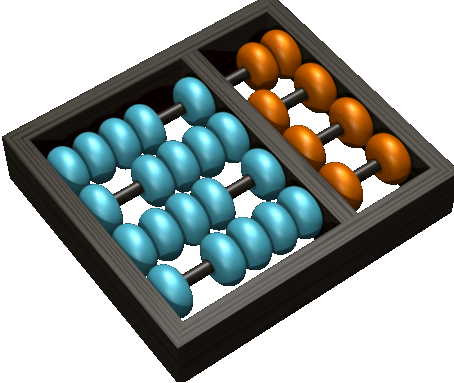
\includegraphics[scale=0.2]{images/logo_ic.png}
        \end{figure}
    \end{column}

    \begin{column}{5cm}
        \begin{figure}
            
\includegraphics[scale=0.4]{images/unicamp-logo.jpg}
        \end{figure}
    \end{column}
\end{columns}

\vspace{0.5cm}

\begin{figure}
    
\includegraphics[scale=1]{images/cnpq.jpg}
\end{figure} }

\end{document}
